\chapter{Timoshenko beam model of a cantilever}

\modinfo{Directory}{TimoshenkoBeamCantilever}
\modinfo{Solvers}{\Idx{BeamSolver3D}}
\modinfo{Tools}{\Idx{ElmerGrid}, \Idx{Python}, \Idx{Gmsh}}
\modinfo{Dimensions}{3D, Steady-state}

\subsection*{Case definition}

In this tutorial, the geometry of a basic cantilever beam is created with Gmsh via its Python interface and simulated with Timoshenko beam elements when the applied force is a constant pressure load. Different numbers of elements for the cantilever are used to demonstrate divergence from the analytical solution for low number of elements. The workflow will be implemented in python and it demonstrates shortly how multiple simulations with different parameters can be created from a pre-existing sif-file.

\subsection*{Requirements}

Before you do this tutorial, you have to do the following things:
\begin{itemize}
   \item install the required python packages (e.g.\ via pip install) found in requirements.txt. If you do not get the exact versions, that should not matter. 
   \item replace in the file create\_geometry.py the variable of the ElmerGrid path
   \item replace in the file total\_workflow.py the variable of the ElmerSolver path
\end{itemize}
We expect the reader to have basic Python skills, but no advanced knowledge except knowing how to run a script and the ability to read the code/syntax.

\subsection*{Workflow}

If you want to see the entire workflow, simply run python total\_workflow.py.  For running its individual parts, run the single subroutines:
\begin{itemize}
    \item \textbf{create\_geometry.py:} Create the geometry via Gmsh and convert it to an Elmer usable format via ElmerGrid. Optional: you can view the geometry via the Gmsh graphical user interface.
    \item \textbf{create\_sif.py:} Take the existing constant\_pressure\_load.sif and modify it for different mesh resolutions for postprocessing files not to overwrite each other.
    \item \textbf{plot\_results.py:} Collect simulations and display them.
\end{itemize}

\subsection*{Geometry Creation}
We import the packages and functions that we need for the task. We need gmsh to create and mesh the geometry, numpy for some basic array functionality (although it could be done without it) and from the subprocess package of the basic libraries of Python the function run to use Elmergrid:
\ttbegin
from subprocess import run

import numpy as np

import gmsh 
\ttend
Enter the path to Elmergrid. If it was added to the system path already, it looks like this
\ttbegin 
elmergrid = r"ElmerGrid"
\ttend
We want to do the geometry creation repeatedly, so we define it as a function of the characteristic mesh length which determines the number of elements in the model and optionally allow the Gmsh graphical user interface (GUI) to be opened to have a final look at the geometry. 
\ttbegin 
def create_geo(lc=1e-2, gui=False):
\ttend
When starting to work on a Gmsh model, you first have to start Gmsh
\ttbegin
gmsh.initialize()
\ttend
and create the empty object 
\ttbegin
gmsh.model()
\ttend
that you will later fill with nodes, lines, surfaces etc.\ that are then meshed. We now create the start and endpoint of our beam at the positions (0,0) and (1,0). 
\ttbegin
i = 0
for x,y in zip([0.,1.],[0.,0.]):
    i = i + 1    
    gmsh.model.geo.addPoint(x, y, 0., lc, i) 
\ttend
Notice that every entity in Gmsh has a tag or index (here i). Indices start always from 1. Next we create a line to connect our nodes. This will later form our physical beam.
\ttbegin
gmsh.model.geo.addLine(1, 2, 1)
\ttend
Before geometric entities can be meshed or manipulated outside the standard Gmsh kernel, they must be synchronized with the Gmsh model creating/updating relevant internal data structures. Synchronizations can be called at any time but they are expensive, so minimize the number of synchronization points for large complicated geometries. 
\ttbegin
gmsh.model.geo.synchronize()
\ttend
In Gmsh, entities are grouped together into Physical Groups to later assign material properties, boundary conditions etc.\ to these. Usually also only the physical groups are explicitly meshed. For each group the dimension of the objects which are to be grouped is first mentioned (0 points, 1 lines, 2 surfaces, 3 bodies), then a list of the tags/ids of the objects and finally a name. Here we define our beam and the point where we apply the boundary condition:
\ttbegin
gmsh.model.addPhysicalGroup(1, [1],name = "beam")
\ttend  
\ttbegin  
gmsh.model.addPhysicalGroup(0, [1], name = "anchor")
\ttend
We then generate a mesh where the dimensionality of the intended mesh must given. As we intend to create line/beam elements, it is 1.
\ttbegin
gmsh.model.mesh.generate(1)
\ttend
As we want to study mesh convergence, we need to know the number of elements. We iterate over all existing Physical Groups, find the ones that are lines by checking the group dimension to be one and count the number of elements tags.
\ttbegin
for phys in gmsh.model.getEntities():
   if phys[0] == 1:
      eltyps, eltags, ndtags = gmsh.model.mesh.getElements(phys[0], 
                                                           phys[1]) 
      nelements = eltags[0].shape[0]
\ttend
We save the number of elements to disk in a simple csv file
\ttbegin
np.savetxt("cantilever-{0}_nelem.csv".format(str(lc)), np.array([nelements]))
\ttend
and save the mesh to the disk as well: 
\ttbegin
filename = "cantilever-{0}.msh".format(str(lc))
gmsh.write(filename)
\ttend
Gmsh automatically infers the format of the file by its ending. Optionally one can start the graphical user interface of Gmsh to inspect the geometry before finishing:
\ttbegin
if gui:
   gmsh.fltk.run()
\ttend 
We clear out the geometry
\ttbegin
gmsh.clear()
\ttend 
and close Gmsh
\ttbegin
gmsh.finalize()
\ttend 
The latter two steps must always be taken as otherwise the geometry is considered open and will linger in the background and may cause strange errors as tags of entities are still assigned and must not be reassigned as it will cause an error. We now need to convert the mesh in Gmsh format to an Elmer friendly one. We do this with ElmerGrid by calling the shell from python
\ttbegin
run([elmergrid, "14", "2", filename], shell=True, check=True)
\ttend
The check flag causes an error if the statement returns an error in the shell. If not present, this program would fail without raising an error. If you encounter problems with the latter statement, you have probably not entered the ElmerGrid path correctly. If for some reason this line does not work despite your best efforts, just comment it out
\ttbegin
#run([elmergrid, "14", "2", filename], shell=True, check=True)
\ttend
and run ElmerGrid by yourself 
\ttbegin
ElmerGrid 14 2 cantilever.msh
\ttend
by adapting the file name accordingly. We now want to see whether this program works, so we enter at the bottom of the program this standard expression
\ttbegin
if __name__ == '__main__':
\ttend 
that ensures, that this routine is only executed when you explicitly call this program file via
\ttbegin
python create_geometry.py
\ttend
and not if you call the function create\_geo from another program. We now perform a simple visual check that everything runs fine
\ttbegin
   lc = 1e0
   create_geo(lc, True)
\ttend
which should result in a geometry with one beam element. Do not get confused as Gmsh also counts the nodes as elements, so its report will mention three. The GUI output should look like Fig. \ref{fig:timoshenko-gmsh-GUI}. 

\begin{figure}[hbt]
  \centerline{\includegraphics[width=1.0\textwidth]{gmsh-GUI}}
  \caption{Output of the Gmsh GUI.} 
  \label{fig:timoshenko-gmsh-GUI}
\end{figure}

\subsection*{Solution Procedure}
We tell Elmer to find the geometric information in the directory cantilever  
\ttbegin
Header
  Mesh DB "." "cantilever"
End
\ttend
and specify the coordinate system, some general output options and the output file in which displacements will be stored:
\ttbegin
Simulation
  Max Output Level = 5
  Coordinate System = Cartesian 3D
  Simulation Type = Steady
  Output Intervals = 1
  Steady State Max Iterations = 1
  Post File = "cantilever.vtu"
End
\ttend 
We will have later to change this automatically. Now we mention which equations, materials and body forces act on body 1
\ttbegin
Body 1
  Equation = 1
  Material = 1
  Body Force = 1
End
\ttend 
which is our only geometric object here. The material data and the geometric data of the beam have to be entered. We make a simplification here, by assuming that we have a beam shape that does not depend on the orientation of the beam with regards to loading, in other words a cylindrical beam:
\ttbegin
Material 1
 Youngs Modulus = Real 2.0e-1
 Shear Modulus = Real 1.0
 Second Moment of Area 2 = Real 1.0
 Second Moment of Area 3 = Real 1.0
 Cross Section Area = Real 1.0
 Torsional Constant = Real 1.0
 Density = 2700.0
End
\ttend 
The density is not needed here.
We specify the constant pressure load as body force acting in y-direction
\ttbegin
Body Force 1
  Body Force 1 = 0.0
  Body Force 2 = 1.0e-2
  Body Force 3 = 0.0
End
\ttend 
and set up the beam solver.
\ttbegin
Equation 1 :: Active Solvers(1) = 1

Solver 1
  Equation = "Timoshenko Beam Equations"
  Procedure = "BeamSolver3D" "TimoshenkoSolver"

  Linear System Solver = "Direct"
End
\ttend 
We can choose the most simple direct solver here as our system is quite small. Solver 2 is just a way to save some scalar data in the file cantilever.dat of the free end to later compare it with the analytic solution. We will have to change the name of the file later as well.
\ttbegin
Solver 2
  Equation = "Save Scalars"
  Exec Solver = After Timestep
  Procedure = "SaveData" "SaveScalars"
  Filename = cantilever.dat
  Variable 1 = U 1
  Variable 2 = U 2
  Variable 3 = U 3
  Variable 4 = Theta 1
  Variable 5 = Theta 2
  Variable 6 = Theta 3
  Save Points(1) = 2
End
\ttend 
We fix the first node in place
\ttbegin
Boundary Condition 1
  Target Nodes(1) = 1
  U 1 = Real 0.0
  U 2 = Real 0.0
  U 3 = Real 0.0
  Theta 1 = Real 0.0
  Theta 2 = Real 0.0
  Theta 3 = Real 0.0
End
\ttend
and are done with the simulation. No other boundary conditions need to be mentioned as everything else is free. Run the simulation by entering 
\ttbegin
ElmerSolver constant_pressure_load.sif
\ttend 
in the command line, and you should find in the directory cantilever a file called cantilever\_t0001.vtu which you can display with ParaView (Fig. \ref{fig:timoshenko-paraview}). 
\begin{figure}[hbt]
  \centerline{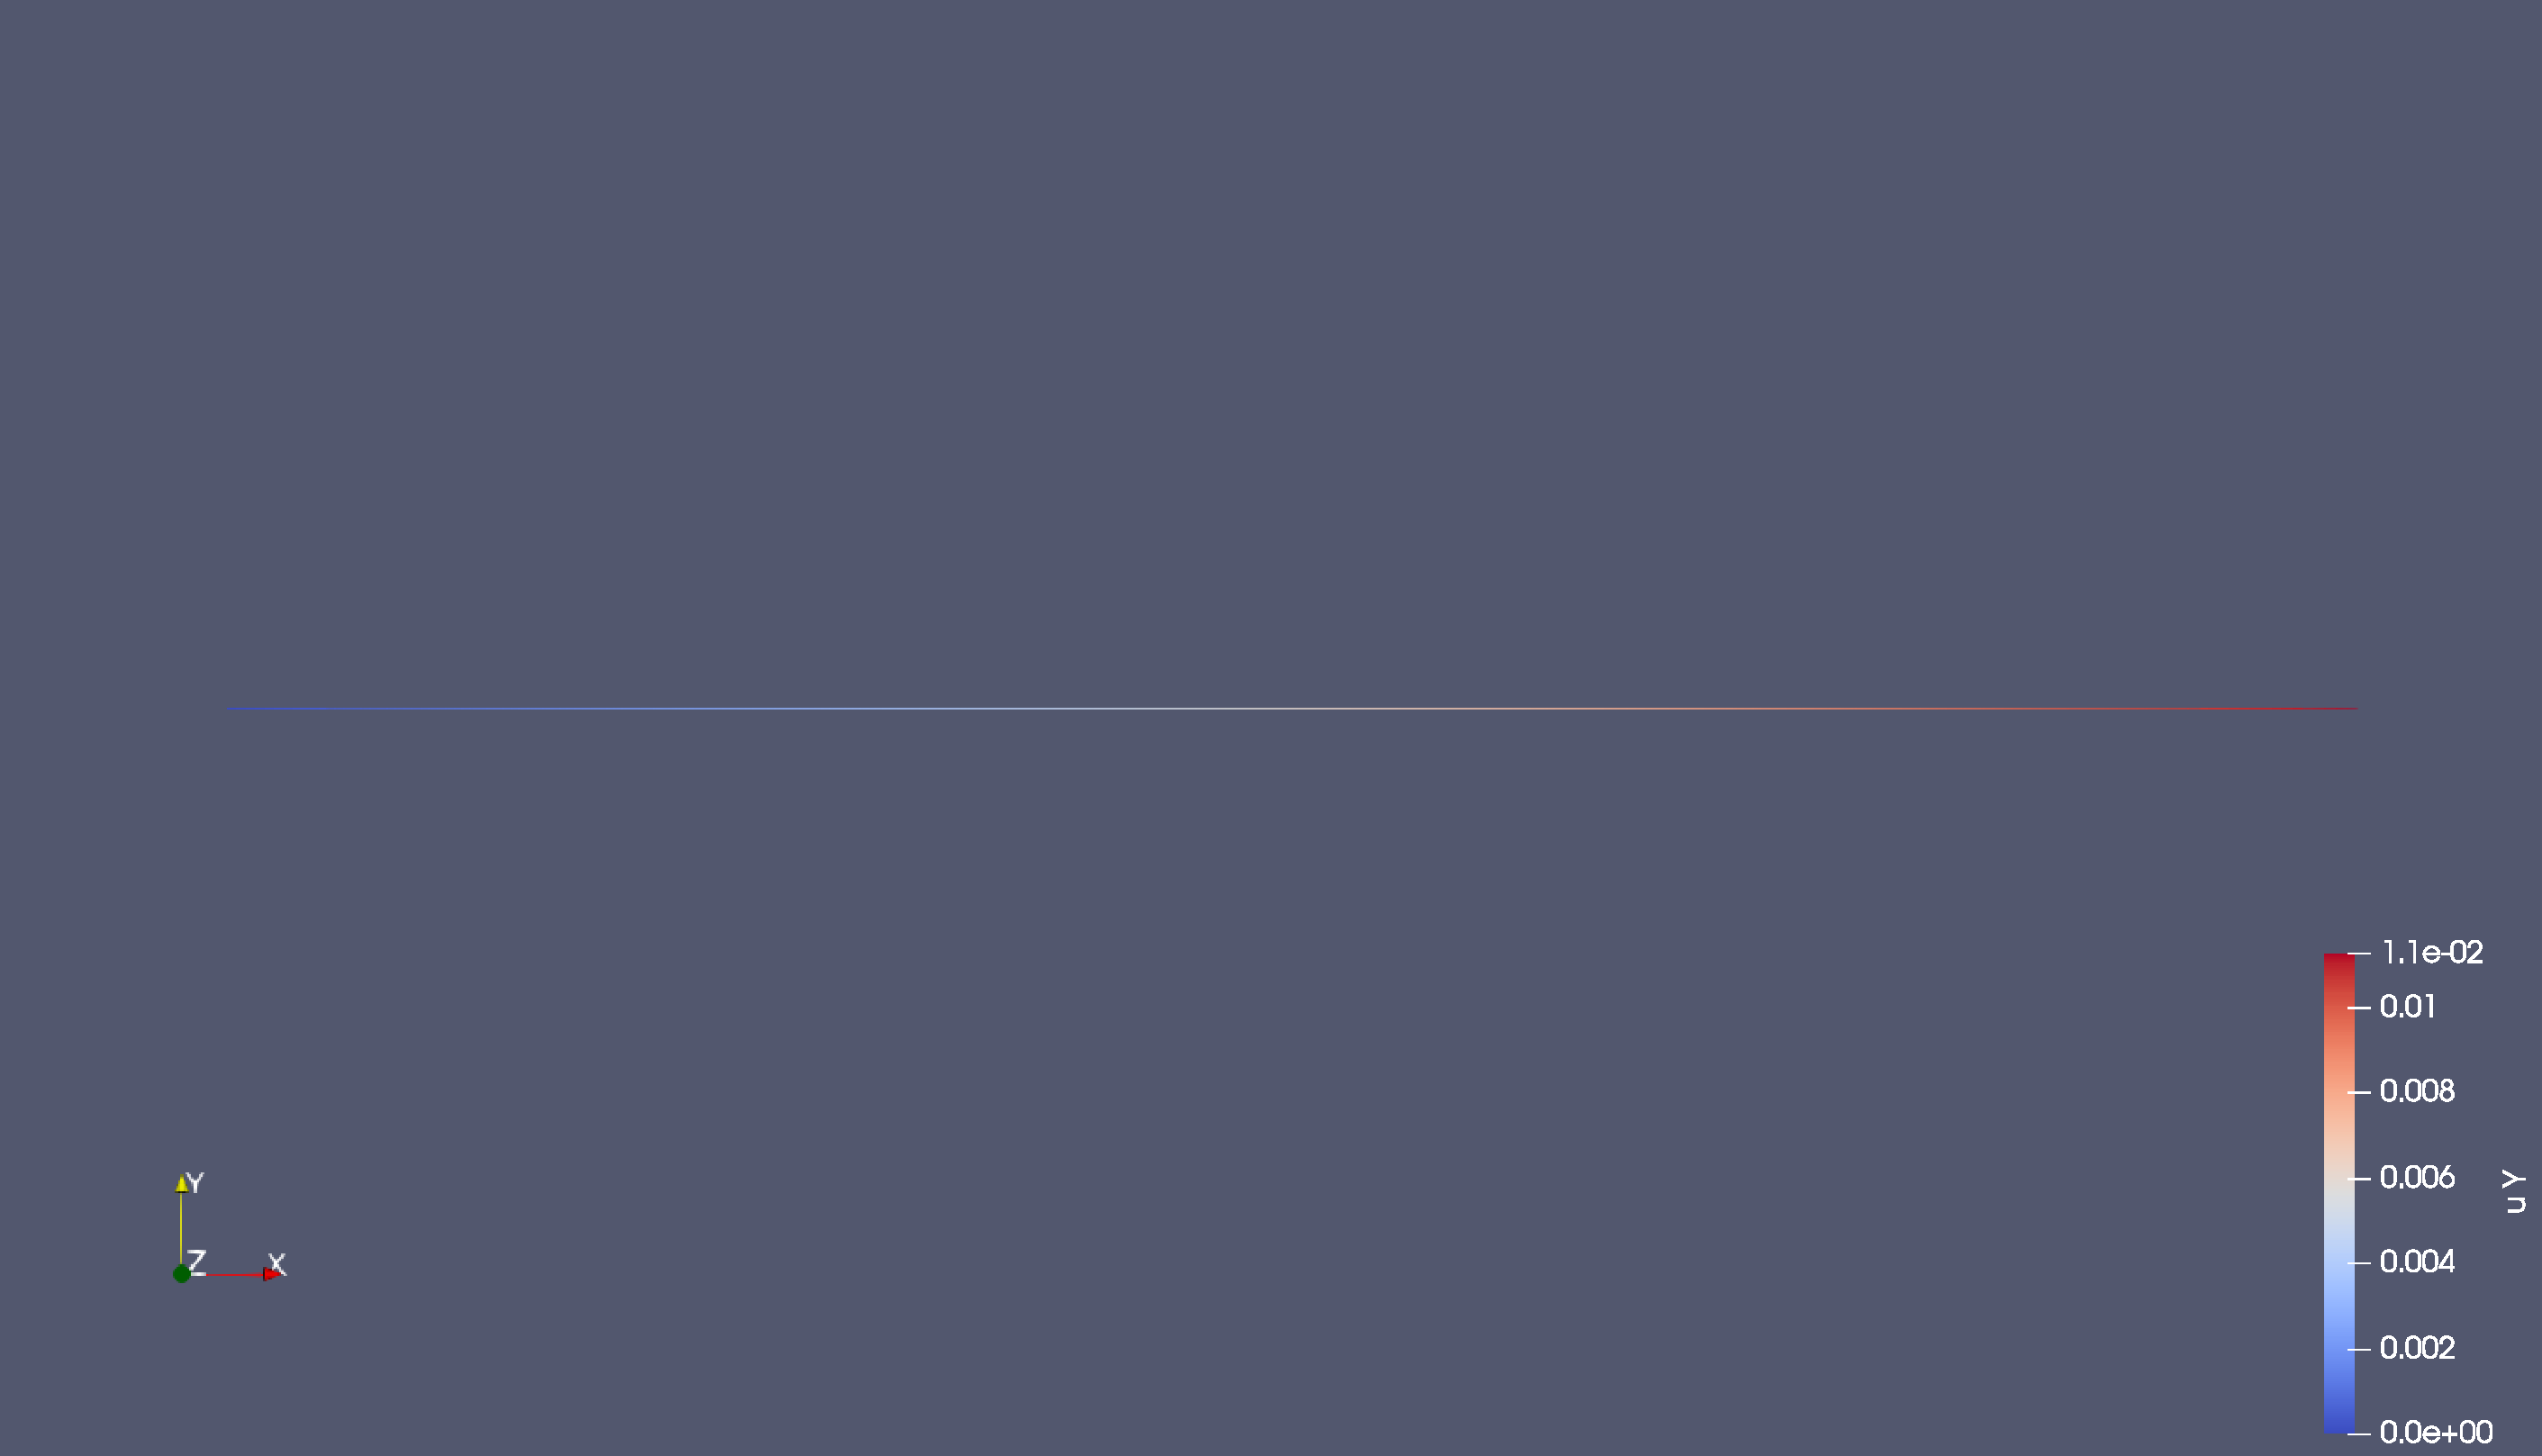
\includegraphics[width=1.0\textwidth]{displacements-paraview.pdf}}
  \caption{Output of ParaView.} 
  \label{fig:timoshenko-paraview}
\end{figure}
\subsection*{Creating New sif-Files}
We do not need to import any packages here, as everything can be done with basic Python functions. We want to update a specific sif file ad replicate it with by changing a few lines and leave 99 \% of the file untouched. Therefore as input for our function we have that file's name, a list of lines that we want to exchange and the replacements of these specific lines. The characteristic mesh length scale is there to change the name of the file. 
\ttbegin
def write_new_sif(file, 
                  search_strings, 
                  replacements,
                  lc):
\ttend 
We read the already existing sif file and all its lines. 
\ttbegin
    with open(file, 'r') as f:
        lines = f.readlines()
\ttend 
We open a new file whose name is a modified version of the already existing sif file.
\ttbegin
   with open(file.split(".")[0]+"-"+str(lc)+".sif", "w") as f:
\ttend
and iterate over all its lines.
\ttbegin
      for line in lines:
\ttend
We check each line whether a string expression is contained in that line. If not, we copy the line. Otherwise we replace it by the corresponding entry in the replacement list
\ttbegin
          flags = [string in line for string in search_strings]
          if any(flags):
             ind = [i for i,flag in enumerate(flags) if flag][0]
             f.write(replacements[ind].format(str(lc)))
          else:
             f.write(line)
    return
\ttend
We quickly test our function with the sif file for the previously generate geometry. 
\ttbegin
if __name__ == '__main__':
    lc = 1e0
\ttend
We exchange the lines that load the geometry, the output file for ParaView and the file containing the displacements of the free end with names changed appropriately for different characteristic mesh length scales.
\ttbegin 
    write_new_sif(file = "constant_pressure_load.sif", 
                  search_strings = ['  Mesh DB "." "cantilever"',
                                    '  Post File = "cantilever.vtu"',
                                    '  Filename = cantilever.dat'], 
                  replacements = ['  Mesh DB "." "cantilever-{0}"\textbackslash n',
                             '  Post File = "cantilever-{0}.vtu"\textbackslash n',
                             '  Filename = cantilever-{0}.dat\textbackslash n'],
                  lc = lc)
\ttend
Check whether the lines have been changed accordingly and move on.
\subsection*{Plotting Results}
We import numpy for some basic array functionality and matplotlib as our standard tool for creating plots in python. 
\ttbegin 
import numpy as np
import matplotlib.pyplot as plt
\ttend 
We define our function for a collection of characteristic length scales and enable optional figure saving as we do not want to dump every figure on our disc.
\ttbegin
def plot\_displacements(lcs,
                       save_fig=False):
\ttend 
For convenience we select a single font size for things like axis labels, etc.
\ttbegin
    font = 14
\ttend 
Set up two lists as collection bags for the number of elements and the displacements and start looping over the characteristic length scales 
\ttbegin
    nelems = []
    displ = []
    for lc in lcs:
\ttend 
We read the number of elements from our previously created csv file when making the geometry, directly put them into the list and do the same for the displacements created by Elmer during the solution process.
\ttbegin
        nelems.append(np.loadtxt("cantilever-{0}_nelem.csv".format(str(lc))))
        displ.append(np.loadtxt("cantilever-{0}.dat".format(str(lc)))[[4,-1]])
\ttend 
After looping we merge the displacements into one array by stacking the list entries on top of each other to receive an array with a variable number of rows and two columns (as we only read two types of displacement). We then split the displacements in two arrays for readability reasons, namely the deflection \(w\) and the rotation \(\Theta\):
\ttbegin
    displ = np.vstack(displ)
    w = displ[:,0]
    theta = displ[:,1]
\ttend 
We create a figure with one row and two columns
\ttbegin 
    fig, axs = plt.subplots(1,2,figsize=(12,8))
\ttend 
and fill each plot with the corresponding element vs.\ displacement data plotted as lines (as an alternative one could use "scatter" instead of plot to have data points instead of lines). 
\ttbegin
    axs[0].plot(nelems,w)
    axs[1].plot(nelems,theta)
\ttend 
We now calculate the analytical solutions and plot them as horizontal red lines to which our simulations should converge with increasing number of elements
\ttbegin
    A,I,G,L,E,f = 1,1,1,1,0.2,1e-2
    axs[0].axhline(y=L**4 * f * ( 1 + 4*E*I / (G*A*L**2) ) / (8*E*I), 
                   color = "r", linestyle="--")
    axs[1].axhline(y=L**3 * f / (6*E*I),
                   color = "r", linestyle="--")
\ttend 
We transform the x-axis to a logarithmic scale as the number of elements may give a large interval and is nonzero
\ttbegin
    axs[0].set_xscale("log")
    axs[1].set_xscale("log")
\ttend 
and adapt the limits of the y scale,
\ttbegin
    axs[0].set_ylim(8e-3,1.2e-2)
    axs[1].set_ylim(8e-3,8.5e-3)
\ttend 
create axis labels
\ttbegin
    axs[0].set_xlabel(r"elements",fontsize=font)
    axs[1].set_xlabel(r"elements",fontsize=font)
    axs[0].set_ylabel(r"deflection \$w\$",fontsize=font)
    axs[1].set_ylabel(r"rotation \$\textbackslash theta\$",fontsize=font)
\ttend 
and allow for the option to save our figure to the disk.
\ttbegin
    if save\_fig:
        plt.savefig("nr-elements-displacements.pdf", format="pdf",
                    bbox_inches="tight")
\ttend 
We now cause our figure to be shown on the screen as so far you should not have seen anything
\ttbegin
    # show the plot as pop up window
    plt.show()
\ttend 
and mark the end of the function by return
\ttbegin
    return 
\ttend 
Strictly speaking the latter is unnecessary as nothing is returned, but helps with readability of the code. As our usual exercise we test our program and you should end up with a single plotted data point.
\ttbegin
if __name__ == '__main__':
    plot_displacements(lcs = np.array([1e0]))
\ttend
\subsection*{Total Workflow for Mesh Convergence Study}
In this section we piece together all our previous programs. We need subprocess.run again for calling Elmersolver and numpy for basic array routines.
\ttbegin
from subprocess import run

from numpy import array
\ttend 
We import all our previously created functions
\ttbegin
from create_geometry import create_geo
from create_sif import write_new_sif
from plot_results import plot_displacements
\ttend 
and add our path to ElmerSolver.
\ttbegin
elmersolver = "ElmerSolver"
\ttend 
We now write the main routine of our solver, create some array with a collection of characteristic length scales that we would like to use and start iteration. (If lc is larger than 1, you will end up with just 1 element, so lc = 1 is the sensible upper bound here)
\ttbegin
if __name__ == '__main__':
    lcs = array([1e0,1e-1,1e-2,1e-3])
    for lc in lcs:
\ttend 
We create the geometry and mesh it with Gmsh to convert it to an Elmer compatible file format
\ttbegin
        create_geo(lc)
\ttend 
and create the corresponding sif file whose geometry input location and its result output files are changed to avoid overwriting previous results.
\ttbegin
        write_new_sif(file = "constant_pressure_load.sif", 
                      search_strings = ['  Mesh DB "." "cantilever"',
                                 '  Post File = "cantilever.vtu"',
                                 '  Filename = cantilever.dat'], 
                      replacements = ['  Mesh DB "." "cantilever-{0}"\textbackslash n',
                                 '  Post File = "cantilever-{0}.vtu"\textbackslash n',
                                 '  Filename = cantilever-{0}.dat\textbackslash n'],
                      lc = lc)
\ttend 
We call Elmer solver to solve the system of equations
\ttbegin
        run([elmersolver,
             "constant_pressure_load-{0}.sif".format(str(lc))],
            shell=True, 
            check=True)
\ttend 
and continue to the next iteration or stop the iteration process. In the end we plot our accumulated results
\ttbegin
    plot_displacements(lcs, True) 
\ttend
which should show a plot similar to Fig.\ \ref{fig:timoshenko-results}. 

\begin{figure}[hbt]
  \centerline{\includegraphics[width=1.0\textwidth]{nr-elements-displacements.pdf}}
  \caption{Collected results.} 
  \label{fig:timoshenko-results}
\end{figure}

\subsection*{Concluding Remarks}

So far this tutorial has presented a minor introduction to the use of the Timoshenko beam solver and applying Elmer in conjunction with Gmsh and also exemplified the usefulness of Python for the construction of workflows to study mesh convergence. For the inexperienced use, we would like to mention that mesh convergence is not usually done with the help of analytical solutions as they are only available in a few cases. Instead one typically analyses the development of the residuals and target outcomes of interest. It goes without saying that if the residuals do not decrease with increasing mesh refinement, you are not converging and you should check the physics and numerics of your problem. 

\vfill
\mbox{}

